\begin{figure}[ht]
    \centering
    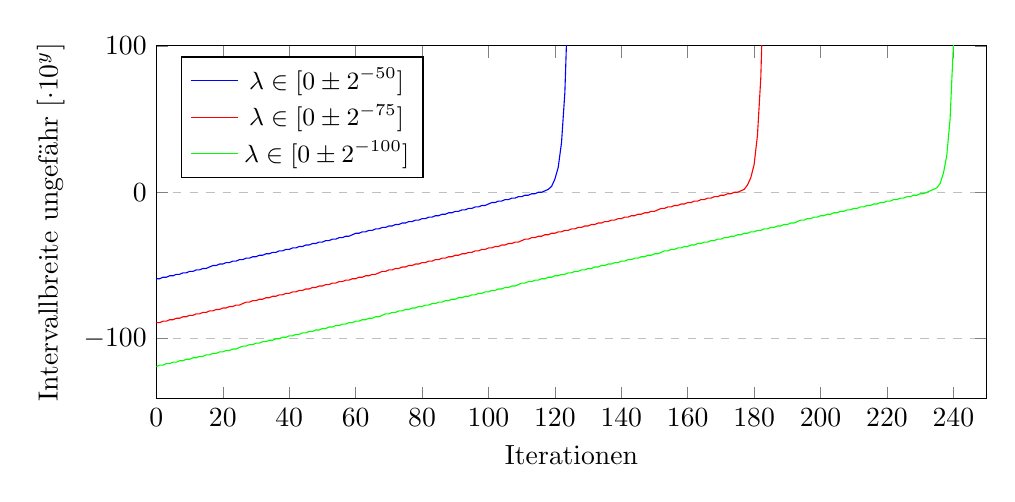
\begin{tikzpicture}
    \begin{axis}[
    width=\textwidth,
    height=0.5\textwidth,
        xlabel={Iterationen},
        ylabel={Intervallbreite ungefähr $[\cdot 10^y ]$},
        legend pos=north west,
        xmin=0,xmax=250,
        ymax=100,
        ymajorgrids=true,
        grid style=dashed,
    ]
    \addplot[
        color=blue,
        ]
        coordinates {
(0,-59) (1,-59) (2,-58) (3,-58) (4,-57) (5,-57) (6,-56) (7,-56) (8,-55) (9,-55) (10,-54) (11,-54) (12,-53) (13,-53) (14,-52) (15,-52) (16,-51) (17,-50) (18,-50) (19,-49) (20,-49) (21,-48) (22,-48) (23,-47) (24,-47) (25,-46) (26,-46) (27,-45) (28,-45) (29,-44) (30,-44) (31,-43) (32,-43) (33,-42) (34,-42) (35,-41) (36,-41) (37,-40) (38,-40) (39,-39) (40,-39) (41,-38) (42,-38) (43,-37) (44,-37) (45,-36) (46,-36) (47,-35) (48,-35) (49,-34) (50,-34) (51,-33) (52,-33) (53,-32) (54,-32) (55,-31) (56,-31) (57,-30) (58,-30) (59,-29) (60,-28) (61,-28) (62,-27) (63,-27) (64,-26) (65,-26) (66,-25) (67,-25) (68,-24) (69,-24) (70,-23) (71,-23) (72,-22) (73,-22) (74,-21) (75,-21) (76,-20) (77,-20) (78,-19) (79,-19) (80,-18) (81,-18) (82,-17) (83,-17) (84,-16) (85,-16) (86,-15) (87,-15) (88,-14) (89,-14) (90,-13) (91,-13) (92,-12) (93,-12) (94,-11) (95,-11) (96,-10) (97,-10) (98,-9) (99,-9) (100,-8) (101,-7) (102,-7) (103,-6) (104,-6) (105,-5) (106,-5) (107,-4) (108,-4) (109,-3) (110,-3) (111,-2) (112,-2) (113,-1) (114,-1) (115,0000) (116,0000) (117,0001) (118,0002) (119,0004) (120,0009) (121,0017) (122,0034) (123,0068) (124,0137) (125,0273) (126,0547) (127,1093) (128,2187) (129,4373) (130,8746)
        };
        \addlegendentry{\small{$\lambda \in [0 \pm 2^{-50}]$}}
        
    \addplot[
        color=red,
        ]
        coordinates {
(0,-89) (1,-89) (2,-88) (3,-88) (4,-87) (5,-87) (6,-86) (7,-86) (8,-85) (9,-85) (10,-84) (11,-84) (12,-83) (13,-83) (14,-82) (15,-82) (16,-81) (17,-81) (18,-80) (19,-80) (20,-79) (21,-79) (22,-78) (23,-78) (24,-77) (25,-77) (26,-76) (27,-75) (28,-75) (29,-74) (30,-74) (31,-73) (32,-73) (33,-72) (34,-72) (35,-71) (36,-71) (37,-70) (38,-70) (39,-69) (40,-69) (41,-68) (42,-68) (43,-67) (44,-67) (45,-66) (46,-66) (47,-65) (48,-65) (49,-64) (50,-64) (51,-63) (52,-63) (53,-62) (54,-62) (55,-61) (56,-61) (57,-60) (58,-60) (59,-59) (60,-59) (61,-58) (62,-58) (63,-57) (64,-57) (65,-56) (66,-56) (67,-55) (68,-54) (69,-54) (70,-53) (71,-53) (72,-52) (73,-52) (74,-51) (75,-51) (76,-50) (77,-50) (78,-49) (79,-49) (80,-48) (81,-48) (82,-47) (83,-47) (84,-46) (85,-46) (86,-45) (87,-45) (88,-44) (89,-44) (90,-43) (91,-43) (92,-42) (93,-42) (94,-41) (95,-41) (96,-40) (97,-40) (98,-39) (99,-39) (100,-38) (101,-38) (102,-37) (103,-37) (104,-36) (105,-36) (106,-35) (107,-35) (108,-34) (109,-34) (110,-33) (111,-32) (112,-32) (113,-31) (114,-31) (115,-30) (116,-30) (117,-29) (118,-29) (119,-28) (120,-28) (121,-27) (122,-27) (123,-26) (124,-26) (125,-25) (126,-25) (127,-24) (128,-24) (129,-23) (130,-23) (131,-22) (132,-22) (133,-21) (134,-21) (135,-20) (136,-20) (137,-19) (138,-19) (139,-18) (140,-18) (141,-17) (142,-17) (143,-16) (144,-16) (145,-15) (146,-15) (147,-14) (148,-14) (149,-13) (150,-13) (151,-12) (152,-11) (153,-11) (154,-10) (155,-10) (156,-9) (157,-9) (158,-8) (159,-8) (160,-7) (161,-7) (162,-6) (163,-6) (164,-5) (165,-5) (166,-4) (167,-4) (168,-3) (169,-3) (170,-2) (171,-2) (172,-1) (173,-1) (174,0000) (175,0000) (176,0001) (177,0002) (178,0005) (179,0010) (180,0019) (181,0039) (182,0078) (183,0156)



        };
        \addlegendentry{\small{$\lambda \in [0 \pm 2^{-75}]$}}
    
        
\addplot[
        color=green,
        ]
        coordinates {
        (0,-119) (1,-118) (2,-118) (3,-117) (4,-117) (5,-116) (6,-116) (7,-115) (8,-115) (9,-114) (10,-114) (11,-113) (12,-113) (13,-112) (14,-112) (15,-111) (16,-111) (17,-110) (18,-110) (19,-109) (20,-109) (21,-108) (22,-108) (23,-107) (24,-107) (25,-106) (26,-105) (27,-105) (28,-104) (29,-104) (30,-103) (31,-103) (32,-102) (33,-102) (34,-101) (35,-101) (36,-100) (37,-100) (38,-99) (39,-99) (40,-98) (41,-98) (42,-97) (43,-97) (44,-96) (45,-96) (46,-95) (47,-95) (48,-94) (49,-94) (50,-93) (51,-93) (52,-92) (53,-92) (54,-91) (55,-91) (56,-90) (57,-90) (58,-89) (59,-89) (60,-88) (61,-88) (62,-87) (63,-87) (64,-86) (65,-86) (66,-85) (67,-85) (68,-84) (69,-83) (70,-83) (71,-82) (72,-82) (73,-81) (74,-81) (75,-80) (76,-80) (77,-79) (78,-79) (79,-78) (80,-78) (81,-77) (82,-77) (83,-76) (84,-76) (85,-75) (86,-75) (87,-74) (88,-74) (89,-73) (90,-73) (91,-72) (92,-72) (93,-71) (94,-71) (95,-70) (96,-70) (97,-69) (98,-69) (99,-68) (100,-68) (101,-67) (102,-67) (103,-66) (104,-66) (105,-65) (106,-65) (107,-64) (108,-64) (109,-63) (110,-62) (111,-62) (112,-61) (113,-61) (114,-60) (115,-60) (116,-59) (117,-59) (118,-58) (119,-58) (120,-57) (121,-57) (122,-56) (123,-56) (124,-55) (125,-55) (126,-54) (127,-54) (128,-53) (129,-53) (130,-52) (131,-52) (132,-51) (133,-51) (134,-50) (135,-50) (136,-49) (137,-49) (138,-48) (139,-48) (140,-47) (141,-47) (142,-46) (143,-46) (144,-45) (145,-45) (146,-44) (147,-44) (148,-43) (149,-43) (150,-42) (151,-42) (152,-41) (153,-40) (154,-40) (155,-39) (156,-39) (157,-38) (158,-38) (159,-37) (160,-37) (161,-36) (162,-36) (163,-35) (164,-35) (165,-34) (166,-34) (167,-33) (168,-33) (169,-32) (170,-32) (171,-31) (172,-31) (173,-30) (174,-30) (175,-29) (176,-29) (177,-28) (178,-28) (179,-27) (180,-27) (181,-26) (182,-26) (183,-25) (184,-25) (185,-24) (186,-24) (187,-23) (188,-23) (189,-22) (190,-22) (191,-21) (192,-21) (193,-20) (194,-19) (195,-19) (196,-18) (197,-18) (198,-17) (199,-17) (200,-16) (201,-16) (202,-15) (203,-15) (204,-14) (205,-14) (206,-13) (207,-13) (208,-12) (209,-12) (210,-11) (211,-11) (212,-10) (213,-10) (214,-9) (215,-9) (216,-8) (217,-8) (218,-7) (219,-7) (220,-6) (221,-6) (222,-5) (223,-5) (224,-4) (225,-4) (226,-3) (227,-3) (228,-2) (229,-2) (230,-1) (231,-1) (232,0000) (233,0001) (234,0002) (235,0003) (236,0006) (237,0013) (238,0025) (239,0050) (240,0101) 


        };
        \addlegendentry{\small{$\lambda \in [0 \pm 2^{-100}]$}}
    
    \end{axis}
    \end{tikzpicture}
    \caption{Größenordnung der Breite des Kernintervalls bei der Berechnung von $x_{250}$ mit Sweeping simple}
    \label{fig:strategy}
\end{figure}
